%%%%%%%%%%%%%%%%%%%%%%%%%%%%%%%%%%%%%%%%%%%%%%%%%%%%%%%%%%%%%%%%%%%%%
% LaTeX Template: Project Titlepage Modified (v 0.1) by rcx
%
% Original Source: http://www.howtotex.com
% Date: November 2017
% 
% This is a title page template which be used for articles & reports.
% 
% This is the modified version of the original Latex template from
% aforementioned website.
% 
%%%%%%%%%%%%%%%%%%%%%%%%%%%%%%%%%%%%%%%%%%%%%%%%%%%%%%%%%%%%%%%%%%%%%%

\documentclass[12pt]{report}
\usepackage[a4paper]{geometry}
\usepackage[myheadings]{fullpage}
\usepackage{fancyhdr}
\usepackage{lastpage}
\usepackage{graphicx, wrapfig, subcaption, setspace, booktabs}
\usepackage[T1]{fontenc}
\usepackage[font=small, labelfont=bf]{caption}
\usepackage{fourier}
\usepackage[protrusion=true, expansion=true]{microtype}
\usepackage[english]{babel}
\usepackage{sectsty}
\usepackage{url, lipsum}


\newcommand{\HRule}[1]{\rule{\linewidth}{#1}}
\onehalfspacing{}
\setcounter{tocdepth}{5}
\setcounter{secnumdepth}{5}

%-------------------------------------------------------------------------------
% HEADER & FOOTER
%-------------------------------------------------------------------------------
\pagestyle{fancy}
\fancyhf{}
\setlength\headheight{15pt}
\fancyhead[L]{Student ID\@: 101006753}
\fancyhead[R]{Carleton University}
\fancyfoot[R]{Page \thepage\ of~\pageref{LastPage}}
%-------------------------------------------------------------------------------
% TITLE PAGE
%-------------------------------------------------------------------------------

\begin{document}

\title{ \HRule{0.5pt} \\
		\LARGE \textbf{\uppercase{Proof on the Uniqueness of the Sicherman dice}}
		\HRule{2pt} \\ [0.5cm]
		\normalsize \today \vspace*{5\baselineskip}}

\date{}

\author{
		Name: Robert Lech \\
        Student ID\@: 101006753 \\ 
		Carleton University \\
		Department of Mathematics }

\maketitle

%-------------------------------------------------------------------------------
% Section title formatting
\sectionfont{\scshape}
%-------------------------------------------------------------------------------

%-------------------------------------------------------------------------------
% BODY
%-------------------------------------------------------------------------------

\section*{Introduction}
Often times, the jump from the abstract to the real-life application is what makes a proof so interesting. We
commonly use number theory and group theory to prove properties of encryption methods. We use the
representation theory of finite groups to infer structural information about molecules in chemistry. Lastly,
we note that problems in discrete probability rely heavily on techniques developed in combinatorics.
Generally, it's the ability to connect the real-world problems to questions in mathematics is what really
allows us to properly tackle them in systematic, and sometimes simple, ways. For the purposes of our paper, we
attempt to do exactly this to a well-known question in probability.

In this paper, we pose the problem, ``Suppose we have a pair of 1 to 6 dice. What other pair\@(s) of dice are
there that provide the same probability distribution?'' Suppose we had a die labelled, $1,2,2,3,3,4$ and
another labelled $1,3,4,5,6,8$. It's clear from Figure~\ref{fig:wikipedia_table} that there is 1 way for a
pair of dice to be rolled and produce a sum of 2, 2 ways to produce a sum of 3, and so on. Now, suppose we
have a different pair of dice. Therefore, we can conclude that both pairs of dice have the same probability
distribution when rolled. However, what's not as immediately clear is that this odd pair of dice (now called
the \textit{Sicherman dice}) is the only other pair of 6-sided dice, with positive labels, with this exact
probability distribution.

\begin{figure}[h]
  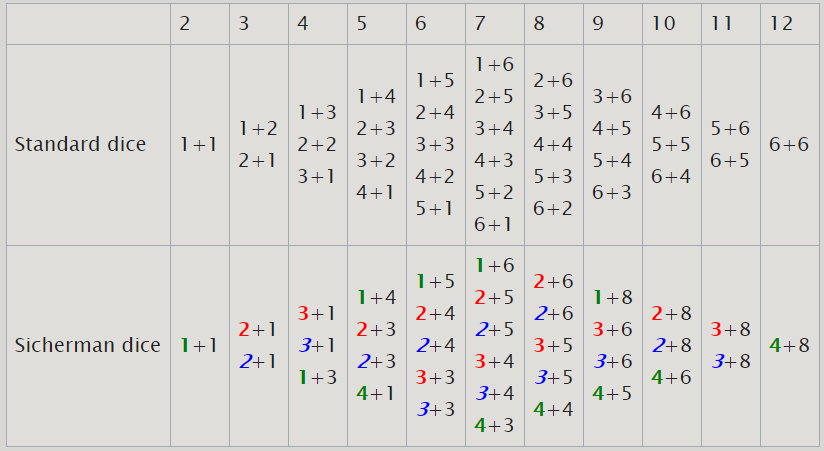
\includegraphics[width=\linewidth]{images/wikipedia_table.png}
  \caption{A table showing that the probability distribution of both dice are the same.}
  \label{fig:wikipedia_table}
\end{figure}

We'll prove this by employing the Unique Factorization Theorem. After this, we'll then apply this to three
other scenarios: a scenario with two tetrahedral dice, a scenario with three cubic dice, and a scenario with
two octahedral dice. We then conclude by restating just how powerful and general this technique is. 

%-------------------------------------------------------------------------------
% Background Information
%-------------------------------------------------------------------------------

\section*{Background Information}
In this section, we state all the algebraic definitions necessary. We start from the very beginning and work
our way forward. We let $G$ be a set together with a binary operation which assigns an ordered pair $(a,b)$ of
elements in $G$ to an element denoted $ab$. We say $G$ is a group under this operation if the following three
properties are satisfied: associativity, the existence of an identity element, and for each element, the
existence of an inverse of that element. Moreover, a group is \textit{Abelian} if the elements commute. We now
build upon this notion of a group by introducing our definition of a \textit{ring}. A \textit{ring} is a set
with two binary operations, addition ((denoted by $(a+b)$) and multiplication (denoted $ab$) such that a ring
forms an Abelian group under addition and having an associative multiplication that is left and right
distributive over addition. When a ring contains an identity element under multiplication, we call it the
\textit{unity}. We take a step forward and define an \textit{integral domain} is a commutative ring with unity
and no \textit{zero-divisors}; that is, no non-zero elements $a,b$ such that $ab=0$. Lastly, we say that if a
non-zero element of a ring has a multiplicative inverse, we say that it is a \textit{unit}. 

We now introduce our rings of interest. Let $R$ be a commutative ring. Then
$R[x]=\{ a_{n}x + \cdots + a_{0} | a_{i}\in R\}$ is called the \textit{ring of polynomials over $R$ in the
indeterminate $x$}. We're interested in $Z[x]$ under ordinary addition and multiplication, which is known to
be an integral domain since $Z$ is an integral domain. From this definition, we can define a particular type
of polynomial. Let $D$ be an integral domain. Let $f(x)\in D[x]$ be a non-zero or non-unit over $D[x]$. If for
every $f(x)=g(x)h(x)$, either $g(x)$ or $h(x)$ is unit, then $f(x)$ is \textit{irreducible}. Otherwise, it's
\textit{reducible}. With all these definitions in place, we introduce the final ingredient we'll need to prove
the uniqueness of the Sicherman dice. This is the \textit{Unique Factorization Theorem} which claims that
every polynomial in $Z[x]$ can be factored into the form
$b_{1}b_{2}\ldots b_{s}p_{1}(x)p_{2}(x)\ldots p_{m}(x)$ where $b_{i}$'s are irreducible polynomials of degree
$0$ and $p_{i}(x)$'s are irreducible polynomials of positive degree. Moreover, this factorization is unique
(which the only differences being that another factoring my have different signs in front of each polynomial).
With this all in place, we're ready to tackle our problem.

%-------------------------------------------------------------------------------
% THE PROBLEM
%-------------------------------------------------------------------------------
\section*{The Problem}
To begin the proof, we find a correspondence between summing dice and polynomials. We note that two dice
having a sum of 6 would imply the dice being rolled had values (5,1), (4,2), (3,3), (2,4), or (1,5). Now
suppose we look at $R(x)R(x)=(x^{6}+x^{5}+x^{4}+x^{3}+x^{2}+x^{1})(x^{6}+x^{5}+x^{4}+x^{3}+x^{2}+x^{1})$. We
observe that to pick the term $x^{6}$ in this product, we have to choose them in the following ways:
$x^{5}x^{1}$, $x^{4}x^{2}$, $x^{3}x^{3}$, $x^{2}x^{4}$, or $x^{1}x^{5}$. So there is a clear correspondence
here between the labels of dice whose sum is 6, and the pairs of terms whose products are six. This
correspondence is one to one (that is, any two dice with the same same should have the same correspondence).
Moreover, it's valid for all sums and dice -- including the Sicherman dice and any other potential dice (of
course, we'll show there aren't any others). We'll do this using a constructive argument, of sorts.

Suppose we have two sequences: $A=$ $a_{1}$, $a_{2}$, $a_{3}$, $a_{4}$, $a_{5}$, $a_{6}$ and $B=$ $b_{1}$,
$b_{2}$, $b_{3}$, $b_{4}$, $b_{5}$, $b_{6}$. Let these be the two sequences of positive integer labels for the
faces of pairs of cubes with the property that the probability of rolling any particular sum with these dice
(we'll call them \textit{weird dice}) is the same probability of rolling that sum with ordinary dice labelled
1 through 6. Therefore, as an example, we should also be able to choose 5 tuples $(a_{i_{1}}, b_{j_{1}})$,
$(a_{i_{2}}, b_{j_{2}})$, $(a_{i_{3}}, b_{j_{3}})$, $(a_{i_{4}}, b_{j_{4}})$, $(a_{i_{5}}, b_{j_{5}})$, such
that $a_{i_{s}} \in A$ and $b_{j_{t}} \in B$. Moreover, we should have that the product of two polynomials
$P(x)Q(x)=(x^{a_{6}}+x^{a_{5}}+x^{a_{4}}+x^{a_{3}}+x^{a_{2}}+x^{a_{1}})
(x^{b_{6}}+x^{b_{5}}+x^{b_{4}}+x^{b_{3}}+x^{b_{2}}+x^{b_{1}})$
should give us 5 pairs of terms who whose products is also $x^{6}$. Therefore, we can assume
$(R(x))^{2}=P(x)Q(x)$.

Therefore, now that we're done setting up the equation, we can focus on solving for the possible $a$'s and
$b$'s. We note from the Unique Factorization Theorem that our polynomial factors uniquely like so:
$x^{6}+x^{5}+x^{4}+x^{3}+x^{2}+x^{1} = (x)(x+1)(x^{2}+x+1)(x^{2}-x+1)$ and so
$(x^{6}+x^{5}+x^{4}+x^{3}+x^{2}+x^{1})^2 = (x)^{2}(x+1)^{2}(x^{2}+x+1)^{2}(x^{2}-x+1)^{2}$. However, this
implies $P(x)=(x)^{q}(x+1)^{r}(x^{2}+x+1)^{t}(x^{2}-x+1)^{u}$ where $0\leq q,r,t,u \leq 2$. The bounds are
there because the exponents can't possibly be negative, and $P(x)$ can't possibly introduce more of the same
irreducible polynomials then $(R(x))^2$ introduced.

We now restrict the possibilities for these four parameters by evaluating $P(0)$ and $P(1)$ in two ways.
Firstly, note $P(1)=1^{a_{6}}+1^{a_{5}}+1^{a_{4}}+1^{a_{3}}+1^{a_{2}}+1^{a_{1}}=6$. Moreover,
$P(1)=1^{q}2^{r}3^{t}1^{u}=2^{r}3^{t} \stackrel{!}{=} 6$. Therefore, $r=t=1$. So we have that
$P(x)=(x)^{q}(x+1)(x^{2}+x+1)(x^{2}-x+1)^{u}$. Now, we similarly note that
$P(0)=0^{a_{6}}+0^{a_{5}}+0^{a_{4}}+0^{a_{3}}+0^{a_{2}}+0^{a_{1}}=0$. Moreover,
$P(0)=0^{q}*1*1*1^{u} \stackrel{!}{=} 0$. This implies $q \neq 0$. Now, we'd like to show that $q$ cannot be
2. Suppose, for a contradiction, $q=2$ and $u=0$. Then
$P(x)=(x)^{2}(x+1)(x^{2}+x+1)=x^{5}+2x^{4}+2x^{3}+x^{2}$. That is, the first die should be labelled
$5,4,4,3,3,2$. This implies $Q(x)=(x+1)(x^{2}+x+1)(x^{2}-x+1)^{2}=x^{7}+x^{5}+x^{4}+x^{3}+x^{2}+x^{0}$ and so
the second die should be labelled $7,5,4,3,2,0$. However, we disallow labels of $0$ so this is not allowed.
This occurs similarly for when $u\in \{1,2\}$. Therefore, $q$ cannot be $2$, and so $q=1$. Therefore, we have
that $q=r=t=1$ and $u\in \{0,1,2\}$. So let's not consider the possibilities:

\begin{enumerate}
\item Suppose $u=0$. Then $P(x)=(x)(x+1)(x^{2}+x+1)=x^{4}+2x^{3}+2x^{2}+x^{1}$ and so the die labels are $4,3,3,2,2,1$ -- a Sicherman die.
\item Suppose $u=1$. Then $P(x)=(x)(x+1)(x^{2}+x+1)(x^{2}-x+1)=x^{6}+x^{5}+x^{4}+x^{3}+x^{2}+x^{1}$ and so the die labels are $6,5,4,3,2,1$ -- an ordinary die.
\item Suppose $u=2$. Then $P(x)=(x)(x+1)(x^{2}+x+1)(x^{2}-x+1)^{2}=x^{8}+x^{6}+x^{5}+x^{4}+x^{3}+x^{1}$ and so the die labels are $8,6,5,4,3,1$ -- the other Sicherman die.
\end{enumerate}

Therefore, choose $P(x)$ such that $q=r=t=1$ and $u=0$ and $Q(x)$ such that $q=r=t=1$ and $u=2$. Then these
represent dice with the same probability distribution of an ordinary pair of dice. Moreover, this shows that
the Sicherman dice are the \textit{only} other pair of dice that have this property.

%-------------------------------------------------------------------------------
% ADDITIONAL APPLICATIONS
%-------------------------------------------------------------------------------
\section*{Additional Applications}
We can use this same approach to see what other `weird dice' we can create. We'll tackle this in three
different scenarios: a scenario with two tetrahedral dice, a scenario with three cubic dice, and a scenario
with two octahedral dice.

\subsection*{Weird Tetrahedral Dice}
We start with a pair of tetrahedrons labelled $1,2,3,4$. We'll use the same approach by denoting
$P(x)Q(x)=(x^{a_{4}}+x^{a_{3}}+x^{a_{2}}+x^{a_{1}})
(x^{b_{4}}+x^{b_{3}}+x^{b_{2}}+x^{b_{1}})=(x^{4}+x^{3}+x^{2}+x^{1})^{2}=(x)^{2}(x+1)^{2}(x^{2}+1)^{2}$.
Therefore, we need to solve for $P(x)=(x)^{q}(x+1)^{r}(x^{2}+1)^{s}$ for $q,r,s \in \{0,1,2\}$. We note that
$P(0)=0^{a_{4}}+0^{a_{3}}+0^{a_{2}}+0^{a_{1}}=0$ and $P(0)=(0)^{q}(1)^{r}(1)^{s} \stackrel{!}{=} 0$ which
implies $q \neq 0$. As with the case before, $q=2$ implies we must have a 0 label on the other die, which we
disallow. There, $q=1$. For the second case, we have $P(1)=1^{a_{4}}+1^{a_{3}}+1^{a_{2}}+1^{a_{1}}=4$ and
$P(1)=(1)^{1}(2)^{r}(2)^{s} \stackrel{!}{=} 4 \Rightarrow 2^{r+s}=2^{2} \Rightarrow r+s=2$. Therefore, have
that $s=2-r$ gives us 3 valid dice. 

\begin{enumerate}
\item Suppose $r=0$. Then $P(x)=(x)(x+1)(x^{2}+1)=x^{3}+2x^{2}+x^{1}$ and so the die labels are $3,2,2,1$ -- one weird die.
\item Suppose $r=1$. Then $P(x)=(x)(x+1)(x^{2}+1)=x^{4}+x^{3}+x^{2}+x^{1}$ and so the die labels are $4,3,2,1$ -- an ordinary tetrahedral die.
\item Suppose $r=2$. Then $P(x)=(x)(x+1)(x^{2}+1)=x^{5}+2x^{3}+x^{1}$ and so the die labels are $5,3,3,1$ -- another weird die.
\end{enumerate}

Therefore, choose $P(x)$ such that $q=1$, $r=0$, and $s=2$ and $Q(x)$ such that $q=1$, $r=2$, and $s=0$. Then
these represent dice with labels $3,2,2,1$ and $5,3,3,1$ such that they have the same probability distribution
as that of an ordinary pair of tetrahedral dice. Moreover, this shows that the `weird dice' are the
\textit{only} other pair of tetrahedral dice that have this property.

\subsection*{Weird Triples of Cubic Dice}
We now tackle the question: are there combinations of 3 dice that have the same probability distribution as 3
cubes numbered $1,2,3,4,5,6$? The answer is yes and the approach is almost identical to what we did in the
previous section. We let
$\prod_{i=1}^{3} P_{i}=\prod_{i=1}^{3}(x^{a_{i,6}}+x^{a_{i,5}}+x^{a_{i,4}}+x^{a_{i,3}}+x^{a_{i,2}}+x^{a_{i,1}})=(x^{6}+x^{5}+x^{4}+x^{3}+x^{2}+x^{1})^{3}=((x)(x+1)(x^{2}+x+1)(x^{2}-x+1))^{3}$.
Therefore, we're aiming to solve $P(x)=(x)^{q}(x+1)^{r}(x^{2}+x+1)^{t}(x^{2}-x+1)^{u}$ where
$0\leq q,r,t,u\leq 3$. However, for the exact same reasons as before, evaluating $P(1)$ tells us the $r,t=1$
and evaluating $P(0)$ tells us the $q \neq 0$. We note that setting $q=2,3$ demands at least one of our two
remaining dice have a 0 label, which we disallow. Therefore, $q=1$. What remains is our choice for $u$?   

\begin{enumerate}
\item Suppose $u=0$. Then $P(x)=(x)(x+1)(x^{2}+x+1)=x^{4}+2x^{3}+2x^{2}+x^{1}$ and so the die labels are $4,3,3,2,2,1$ -- a Sicherman die.
\item Suppose $u=1$. Then $P(x)=(x)(x+1)(x^{2}+x+1)(x^{2}-x+1)=x^{6}+x^{5}+x^{4}+x^{3}+x^{2}+x^{1}$ and so the die labels are $6,5,4,3,2,1$ -- an ordinary die.
\item Suppose $u=2$. Then $P(x)=(x)(x+1)(x^{2}+x+1)(x^{2}-x+1)^{2}=x^{8}+x^{6}+x^{5}+x^{4}+x^{3}+x^{1}$ and so the die labels are $8,6,5,4,3,1$ -- the other Sicherman die.
\item Suppose $u=3$. Then $P(x)=(x)(x+1)(x^{2}+x+1)(x^{2}-x+1)^{3}=x^{10}-x^{9}+2x^{8}+x^{6}+x^{5}+2x^{3}-x^{2}+x^{1}$. However, this is not of the form $x^{a_{1,6}}+x^{a_{1,5}}+x^{a_{1,4}}+x^{a_{1,3}}+x^{a_{1,2}}+x^{a_{1,1}}$ where $x^{a_{i,j}} \in \{1,2,\ldots\}$. Therefore, this case is impossible.
\end{enumerate}

Therefore, choose, this allows us to choose two triples of dice: either (a) a pair of Sicherman dice and 1 regular die, or (b) 3 regular dice.

\subsection*{Weird Octahedral Dice}
Lastly, we tackle the question: are there pairs of octahedral dice that have the same probability distribution
as octahedral dice numbered $1,2,3,4,5,6,7,8$? The answer is yes and the approach is almost identical to what
we did in the previous section -- with slightly more work. If we jump ahead, we have our
$R(x)=\sum_{i=1}^{8} x^{i}=(x)(x+1)(x^{2}+1)(x^{4}+1)$. Therefore, our $P(x)$ should be of the form
$(x)^{q}(x+1)^{r}(x^{2}+1)^{t}(x^{4}+1)^{u}$ such that $q,r,t,u \in \{0,1,2\}$. Our usual tricks tell us
$q=1$. However, evaluating $P(1)$ gives us $r+t+u=3$. Therefore, we have 7 choices for $r$, $t$, and $u$.

\begin{enumerate}
\item Suppose $r=0$, $t=1$, and $u=2$. Then $(x)^{1}(x+1)^{0}(x^{2}+1)^{1}(x^{4}+1)^{2}=x^{11}+x^{9}+2x^{7}+2x^{5}+x^{3}+x^{1}$ and so the die labels are $11,9,7,7,5,5,3,1$ -- a weird die
\item Suppose $r=0$, $t=2$, and $u=1$. Then $(x)^{1}(x+1)^{0}(x^{2}+1)^{2}(x^{4}+1)^{1}=x^{9}+2x^{7}+2x^{5}+2x^{3}+x^{1}$ and so the die labels are $9,7,7,5,5,3,3,1$ -- a weird die
\item Suppose $r=1$, $t=0$, and $u=2$. Then $(x)^{1}(x+1)^{1}(x^{2}+1)^{0}(x^{4}+1)^{2}=x^{10}+x^{9}+2x^{6}+2x^{5}+x^{2}+x^{1}$ and so the die labels are $10,9,6,6,5,5,2,1$ -- a weird die
\item Suppose $r=1$, $t=1$, and $u=1$. Then $(x)^{1}(x+1)^{1}(x^{2}+1)^{1}(x^{4}+1)^{1}=x^{8}+x^{7}+x^{6}+x^{5}+x^{4}+x^{3}+x^{2}+x^{1}$ and so the die labels are $8,7,6,5,4,3,2,1$ -- a regular die 
\item Suppose $r=1$, $t=2$, and $u=0$. Then $(x)^{1}(x+1)^{1}(x^{2}+1)^{2}(x^{4}+1)^{0}=x^{6}+x^{5}+2x^{4}+2x^{3}+x^{2}+x^{1}$ and so the die labels are $6,5,4,4,3,3,2,1$ -- a weird die corresponding to the die mentioned in item 3
\item Suppose $r=2$, $t=0$, and $u=1$. Then $(x)^{1}(x+1)^{2}(x^{2}+1)^{0}(x^{4}+1)^{1}=x^{7}+2x^{6}+x^{5}+x^{3}+2x^{2}+x^{1}$ and so the die labels are $7,6,6,5,3,2,2,1$ -- a weird die corresponding to the die mentioned in item 2
\item Suppose $r=2$, $t=1$, and $u=0$. Then $(x)^{1}(x+1)^{2}(x^{2}+1)^{1}(x^{4}+1)^{0}=x^{5}+2x^{4}+2x^{3}+2x^{2}+x^{1}$ and so the die labels are $5,4,4,3,3,2,2,1$ -- a weird die corresponding to the die mentioned in item 1
\end{enumerate}

So our 4 pairs of octahedral dice are:
\begin{enumerate}
\item $(8,7,6,5,4,3,2,1)$ and $(8,7,6,5,4,3,2,1)$
\item $(9,7,7,5,5,3,3,1)$ and $(7,6,6,5,3,2,2,1)$
\item $(10,9,6,6,5,5,2,1)$ and $(6,5,4,4,3,3,2,1)$
\item $(11,9,7,7,5,5,3,1)$ and $(5,4,4,3,3,2,2,1)$
\end{enumerate}

%-------------------------------------------------------------------------------
% CONCLUSION
%-------------------------------------------------------------------------------
\section*{Conclusion}
We finish this project by recalling that the primary tool we used to successfully find, and prove the
uniqueness of, these dice was the Unique Factorization Theorem. That is, what makes this method/proof so
incredible is we used a completely abstract concept from ring theory, that inherently doesn't seem too
applicable to the real world, and applied it directly a real world question. Moreover, this method simply,
efficiently, and reliably solves the problem that would otherwise use an exponentially-growing, brute force
approach to prove. It's very general in that can be applied to dice with large number of size and dice with
varying numbers of faces. These are the reasons for why the method is so powerful. However, these aren't the
only reasons that make a method ``beautiful''.

Another more important facet, from a personal standpoint, that method needs for being beautiful is that it can
make math fun. This is a technique that can be introduced to high-schoolers to learn the importance of
higher-level math in the real world. I know I personally enjoyed applying it to other geometric shapes for
dice that I can create for myself some day, just for fun. This is why I think this proof is so beautiful.

%-------------------------------------------------------------------------------
% REFERENCES
%-------------------------------------------------------------------------------
\section*{References}
\addcontentsline{toc}{section}{References}
Gallian, J. A. (2010). 17. In \textit{Contemporary Abstract Algebra} (7th ed., pp. 314-319). Australia: Brooks/Cole.
\end{document}
